%!TEX root = ../paper.tex

	\begin{figure*}
		\centering
		%!TEX root = ../paper.tex

% Ferdosi 2
\begin{subfigure}{0.23\textwidth}
	\centering
	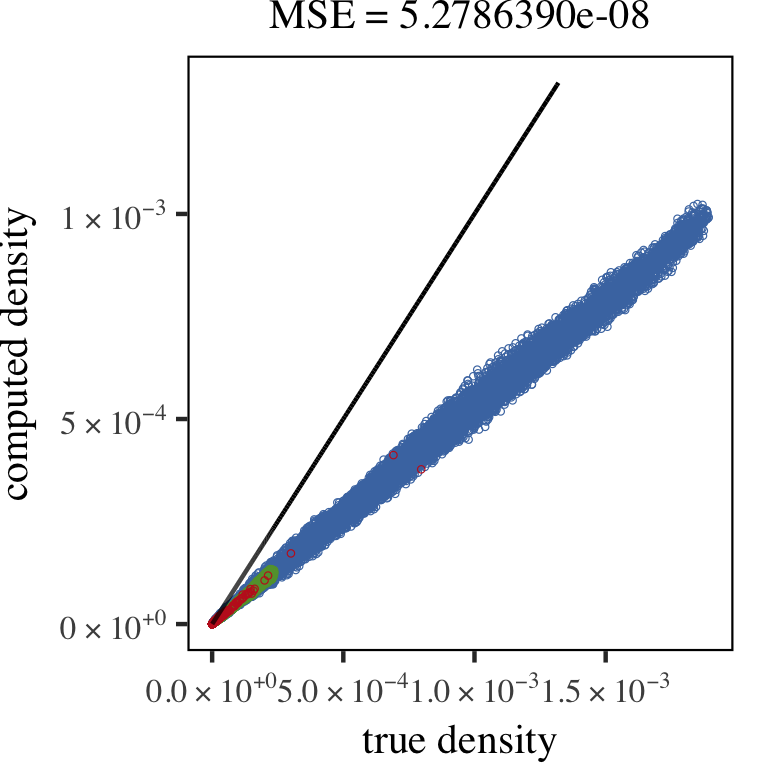
\includegraphics[keepaspectratio=true, width=\textwidth, height=0.23\textheight]{4/img/all/results_ferdosi_2_60000_mbe_silverman}
	\caption{Set \ferdosiTwo, \mbe}
	\label{fig:4:results:mbe:ferdosi2}
\end{subfigure}
\begin{subfigure}{0.23\textwidth}
	\centering
	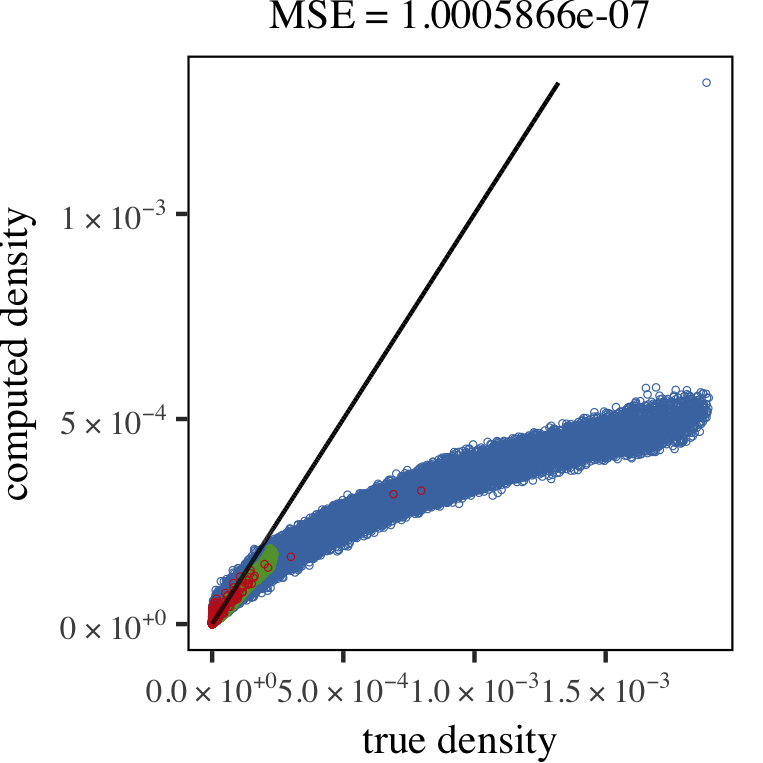
\includegraphics[keepaspectratio=true, width=\textwidth, height=0.23\textheight]{4/img/all/results_ferdosi_2_60000_sambe_silverman}
	\caption{Set \ferdosiTwo, \sambe}
	\label{fig:4:results:sambe:ferdosi2}
\end{subfigure}
% Baakman 2
\begin{subfigure}{0.23\textwidth}
	\centering
	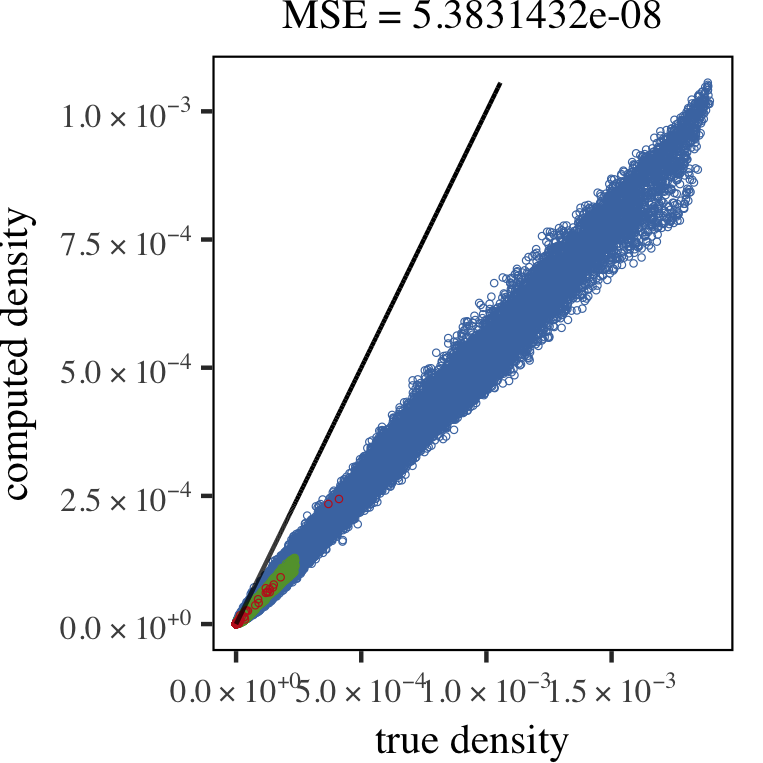
\includegraphics[keepaspectratio=true, width=\textwidth, height=0.23\textheight]{4/img/all/results_baakman_2_60000_mbe_silverman}
	\caption{Set \baakmanTwo, \mbe}
	\label{fig:4:results:mbe:baakman2}
\end{subfigure}
\begin{subfigure}{0.23\textwidth}
	\centering
	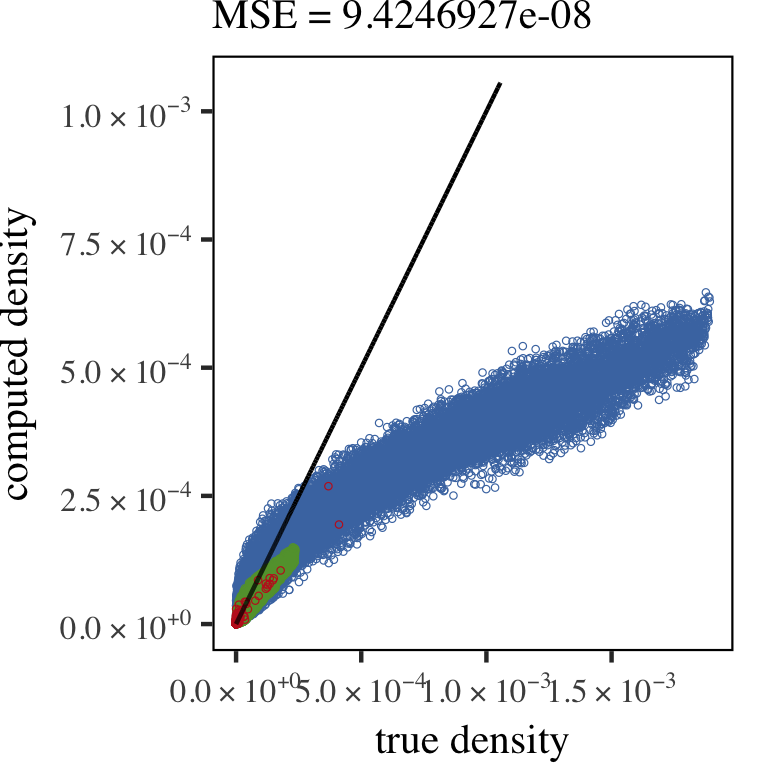
\includegraphics[keepaspectratio=true, width=\textwidth, height=0.23\textheight]{4/img/all/results_baakman_2_60000_sambe_silverman}
	\caption{Set \baakmanTwo, \sambe}
	\label{fig:4:simulated:datasets:sambe:baakman2}
\end{subfigure}
% Ferdosi 3
\begin{subfigure}{0.23\textwidth}
	\centering
	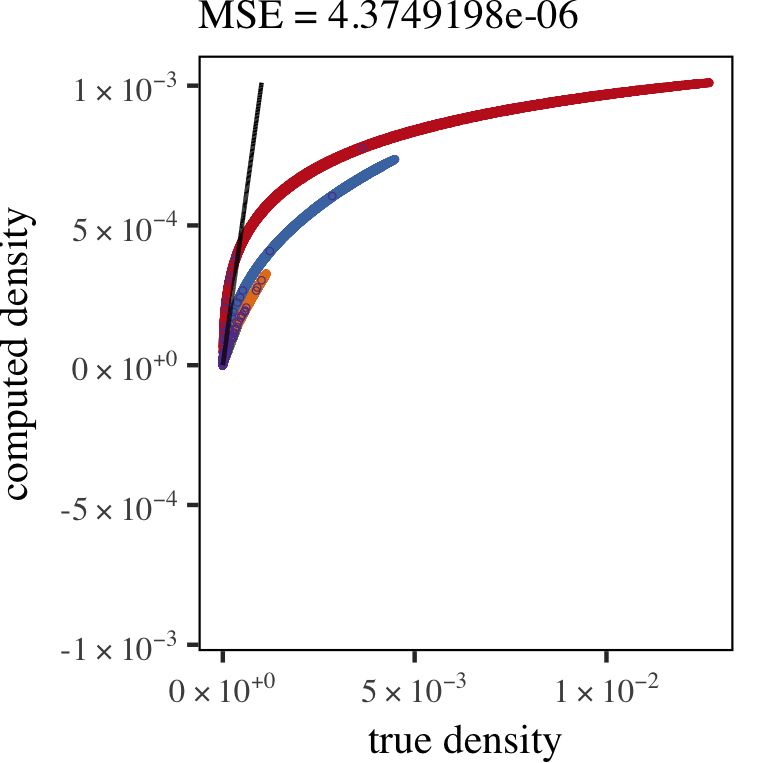
\includegraphics[keepaspectratio=true, width=\textwidth, height=0.23\textheight]{4/img/all/results_ferdosi_3_120000_mbe_silverman.png}
	\caption{Set \ferdosiThree, \mbe}
	\label{fig:4:results:mbe:ferdosi3}
\end{subfigure}
\begin{subfigure}{0.23\textwidth}
	\centering
	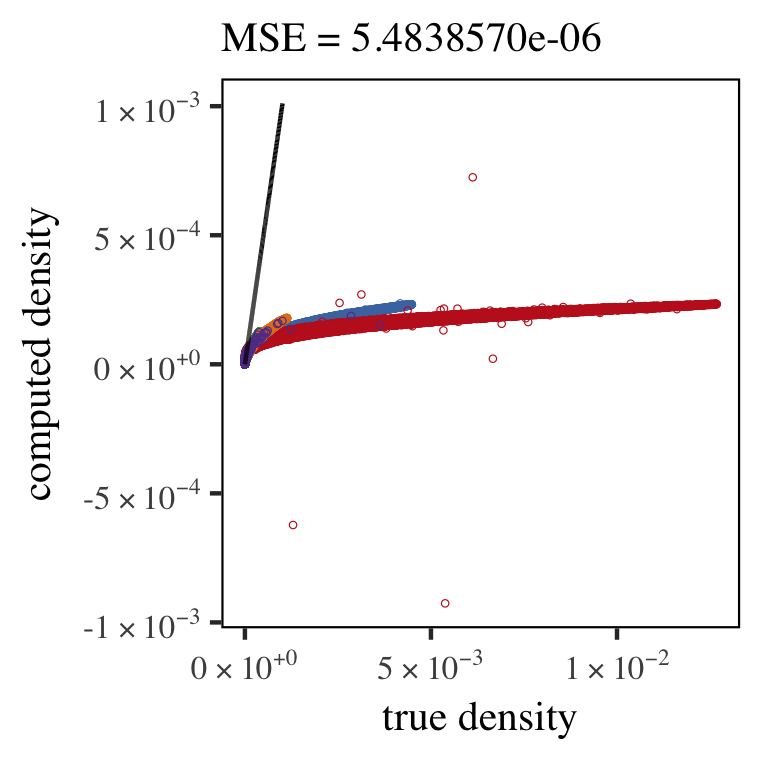
\includegraphics[keepaspectratio=true, width=\textwidth, height=0.23\textheight]{4/img/all/results_ferdosi_3_120000_sambe_silverman}
	\caption{Set \ferdosiThree, \sambe}
	\label{fig:4:simulated:datasets:sambe:ferdosi3}
\end{subfigure}
% Baakman 3
\begin{subfigure}{0.23\textwidth}
	\centering
	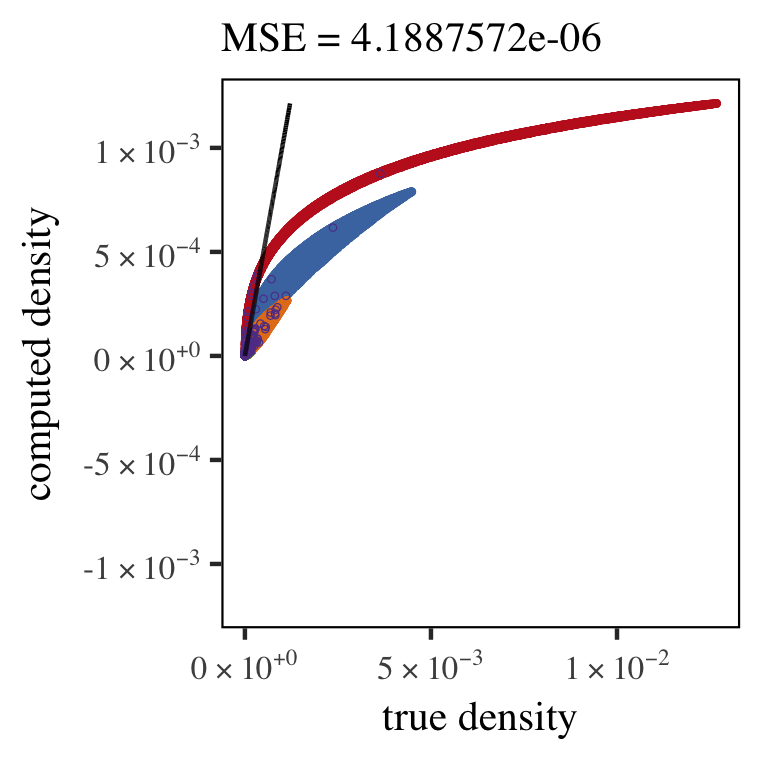
\includegraphics[keepaspectratio=true, width=\textwidth, height=0.23\textheight]{4/img/all/results_baakman_3_120000_mbe_silverman}
	\caption{Set \baakmanThree, \mbe}
	\label{fig:4:results:mbe:baakman3}
\end{subfigure}	
\begin{subfigure}{0.23\textwidth}
	\centering
	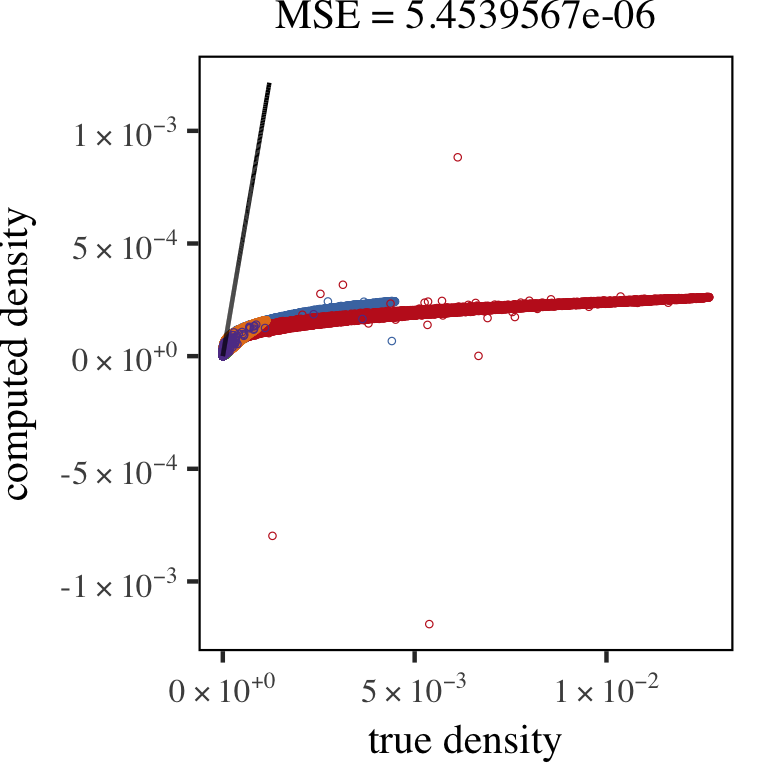
\includegraphics[keepaspectratio=true, width=\textwidth, height=0.23\textheight]{4/img/all/results_baakman_3_120000_sambe_silverman}
	\caption{Set \baakmanThree, \sambe}
	\label{fig:4:results:sambe:baakman3}
\end{subfigure}	
		\caption{Comparative plots for dataset \ferdosiTwoNum, \ferdosiThreeNum, \baakmanTwoNum, and \baakmanThreeNum.}
		\label{fig:4:resuts:multiSphere}
	\end{figure*}

	\todo[inline]{What do we observe in \cref{fig:4:resuts:multiSphere}.}